\documentclass[twocolumn,11pt]{abst}





% タイトル
\title{マルチコプターCFRP立体フレームの製作}

\author{馳 陽大(指導教員 伊藤恒平)}

%\urlstyle{rm}

\setcounter{page}{05}
\lhead{}
\chead{}
\rhead{{\sf 18・203}\\{\bf 機械工学科}}
\lfoot{}
%\cfoot{{\sf-\ M-\thepage \ -}}
\cfoot{
 \ifnum \value{page} <10
  {\sf-\ M-0\thepage \ -}
 \else%
  {\sf-\ M-\thepage \ -}
 \fi%
}
\rfoot{}
\renewcommand{\headrulewidth}{3pt}
%\renewcommand{\footrulewidth}{1pt}



\begin{document}
%\layout
\maketitle
\thispagestyle{fancy}
\pagestyle{fancy}

\setlength{\baselineskip}{5.6truemm}
\kanjiskip=.07zw plus 3pt minus 3pt
\xkanjiskip=.07zw plus 3pt minus 3pt


% 本文

\section{はじめに}
\subsection{研究背景}
近年マルチコプターは,農業,空撮,物資配達,救助といった様々な場面で用いられるようになってきた.遠隔操作が可能で,複数のプロペラや翼を搭載した機体である.現代において更なる技術革新と汎用性が求められている.

\subsection{立体フレーム製作の目的}
本研究室では,マルチコプターを設計から一貫し製作を行ってきた.これまでの研究目標としてきた校内を自律飛行案内するという目標を掲げ活動を行ってきた.中間目標としていた全日本飛行ロボットコンテストに出場し見事に優勝を飾ったが,いくつかの課題も残った.具体的に大会でのミッションとなっていた自動離着陸や,自動八の字飛行ができなかった.また,CFRPフレームにおいても大会規定であった機体重量に対し,自動飛行のためのセンサーなどを搭載していた場合,重量規定を超えてしまっていた.そのためより軽く剛性のあるフレーム製作が最も重要であり必要不可欠であると考えられた.本研究室では平面積層のCFRPフレームに対し,より軽量で剛性のあるフレーム製作を目的とする.そのためこれまでの平面積層ではなく,立体構造のフレーム製作を行った.


\section{平面フレームの製作}
平面フレームを成型するにための型は,ベニヤ板を切り抜いた木枠を用いて製作を行った.

\subsection{型の設計}
型の設計は3DCADを用いて行った.平面積層用の木枠は,ベニヤ板をレーザー加工機を用いて切り抜き,製作を行った.雄型,雌型をそれぞれ設計を行った.

\subsection{レーザー加工機での木枠制作}
カーボンクロスをレーザー加工機を用いて切り出す.レーザー加工機を使用する以前は,ハサミで切って切り出していた.しかしカーボンクロスの繊維が細かく,ささくれてしまい型への積層が困難だった.レーザー加工を行うことで,縁が溶着硬化することができるため積層が綺麗に行うことができる.

\subsection{木型への離型剤吹付け作業}
カーボンクロスの積層には,硬化させるためのエポキシ樹脂を用いる.そのため硬化後に型との離型を容易にするため離型剤を用いる.平面フレーム用の木型には,枠の縁などに塗りやすいようにスプレー式を用いた.

\begin{figure}[htbp]
  \begin{center}
    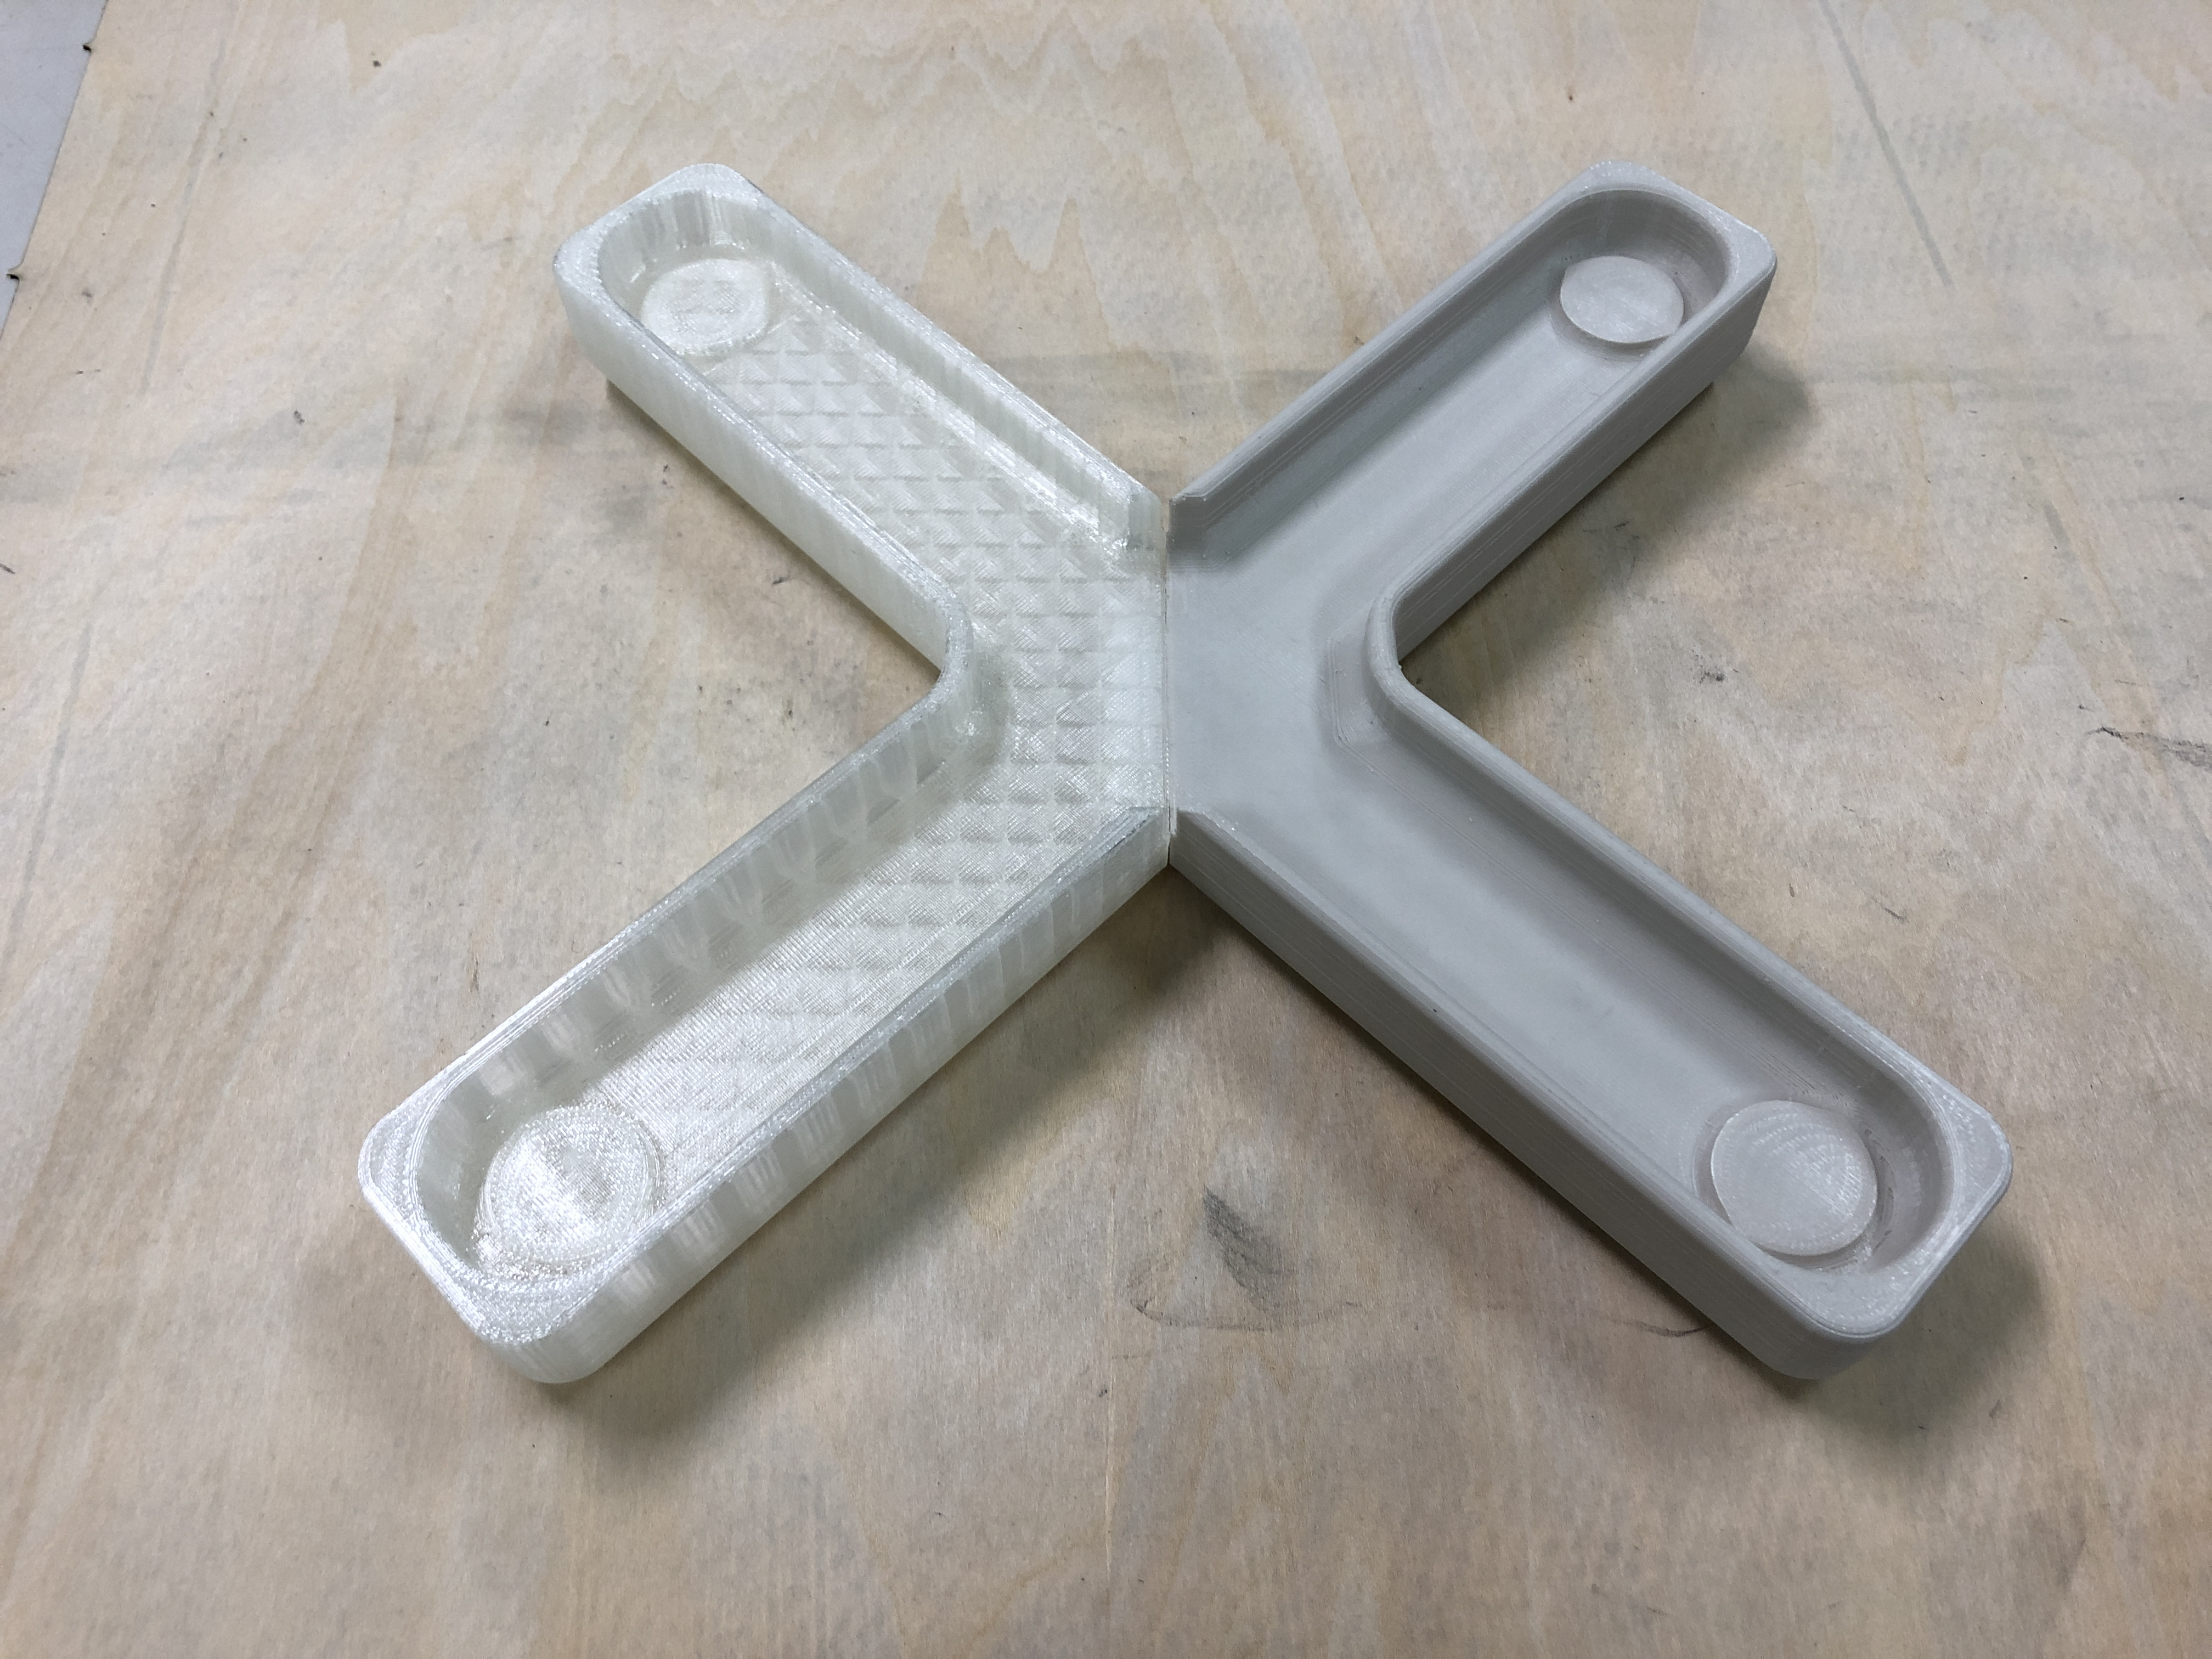
\includegraphics[width=50mm]{img/f.jpg}
    \end{center}
  \caption{離型剤を塗られた型}
 \label{fig:a}
\end{figure}

\subsection{積層作業}
平面積層においては切り出されたふカーボンクロスを枠に合わせ,1枚重ねるごとにエポキシ樹脂を塗り重ね繰り返し行う.重ねる枚数が増えてゆくにつれ塗る硬化剤の量を減らしてゆく.

\subsection{バリ取り,ヤスリ掛け}
24時間以上が経過し完全に硬化したフレームは,やすり掛けを行い完成となる.

\begin{figure}[htbp]
  \begin{center}
    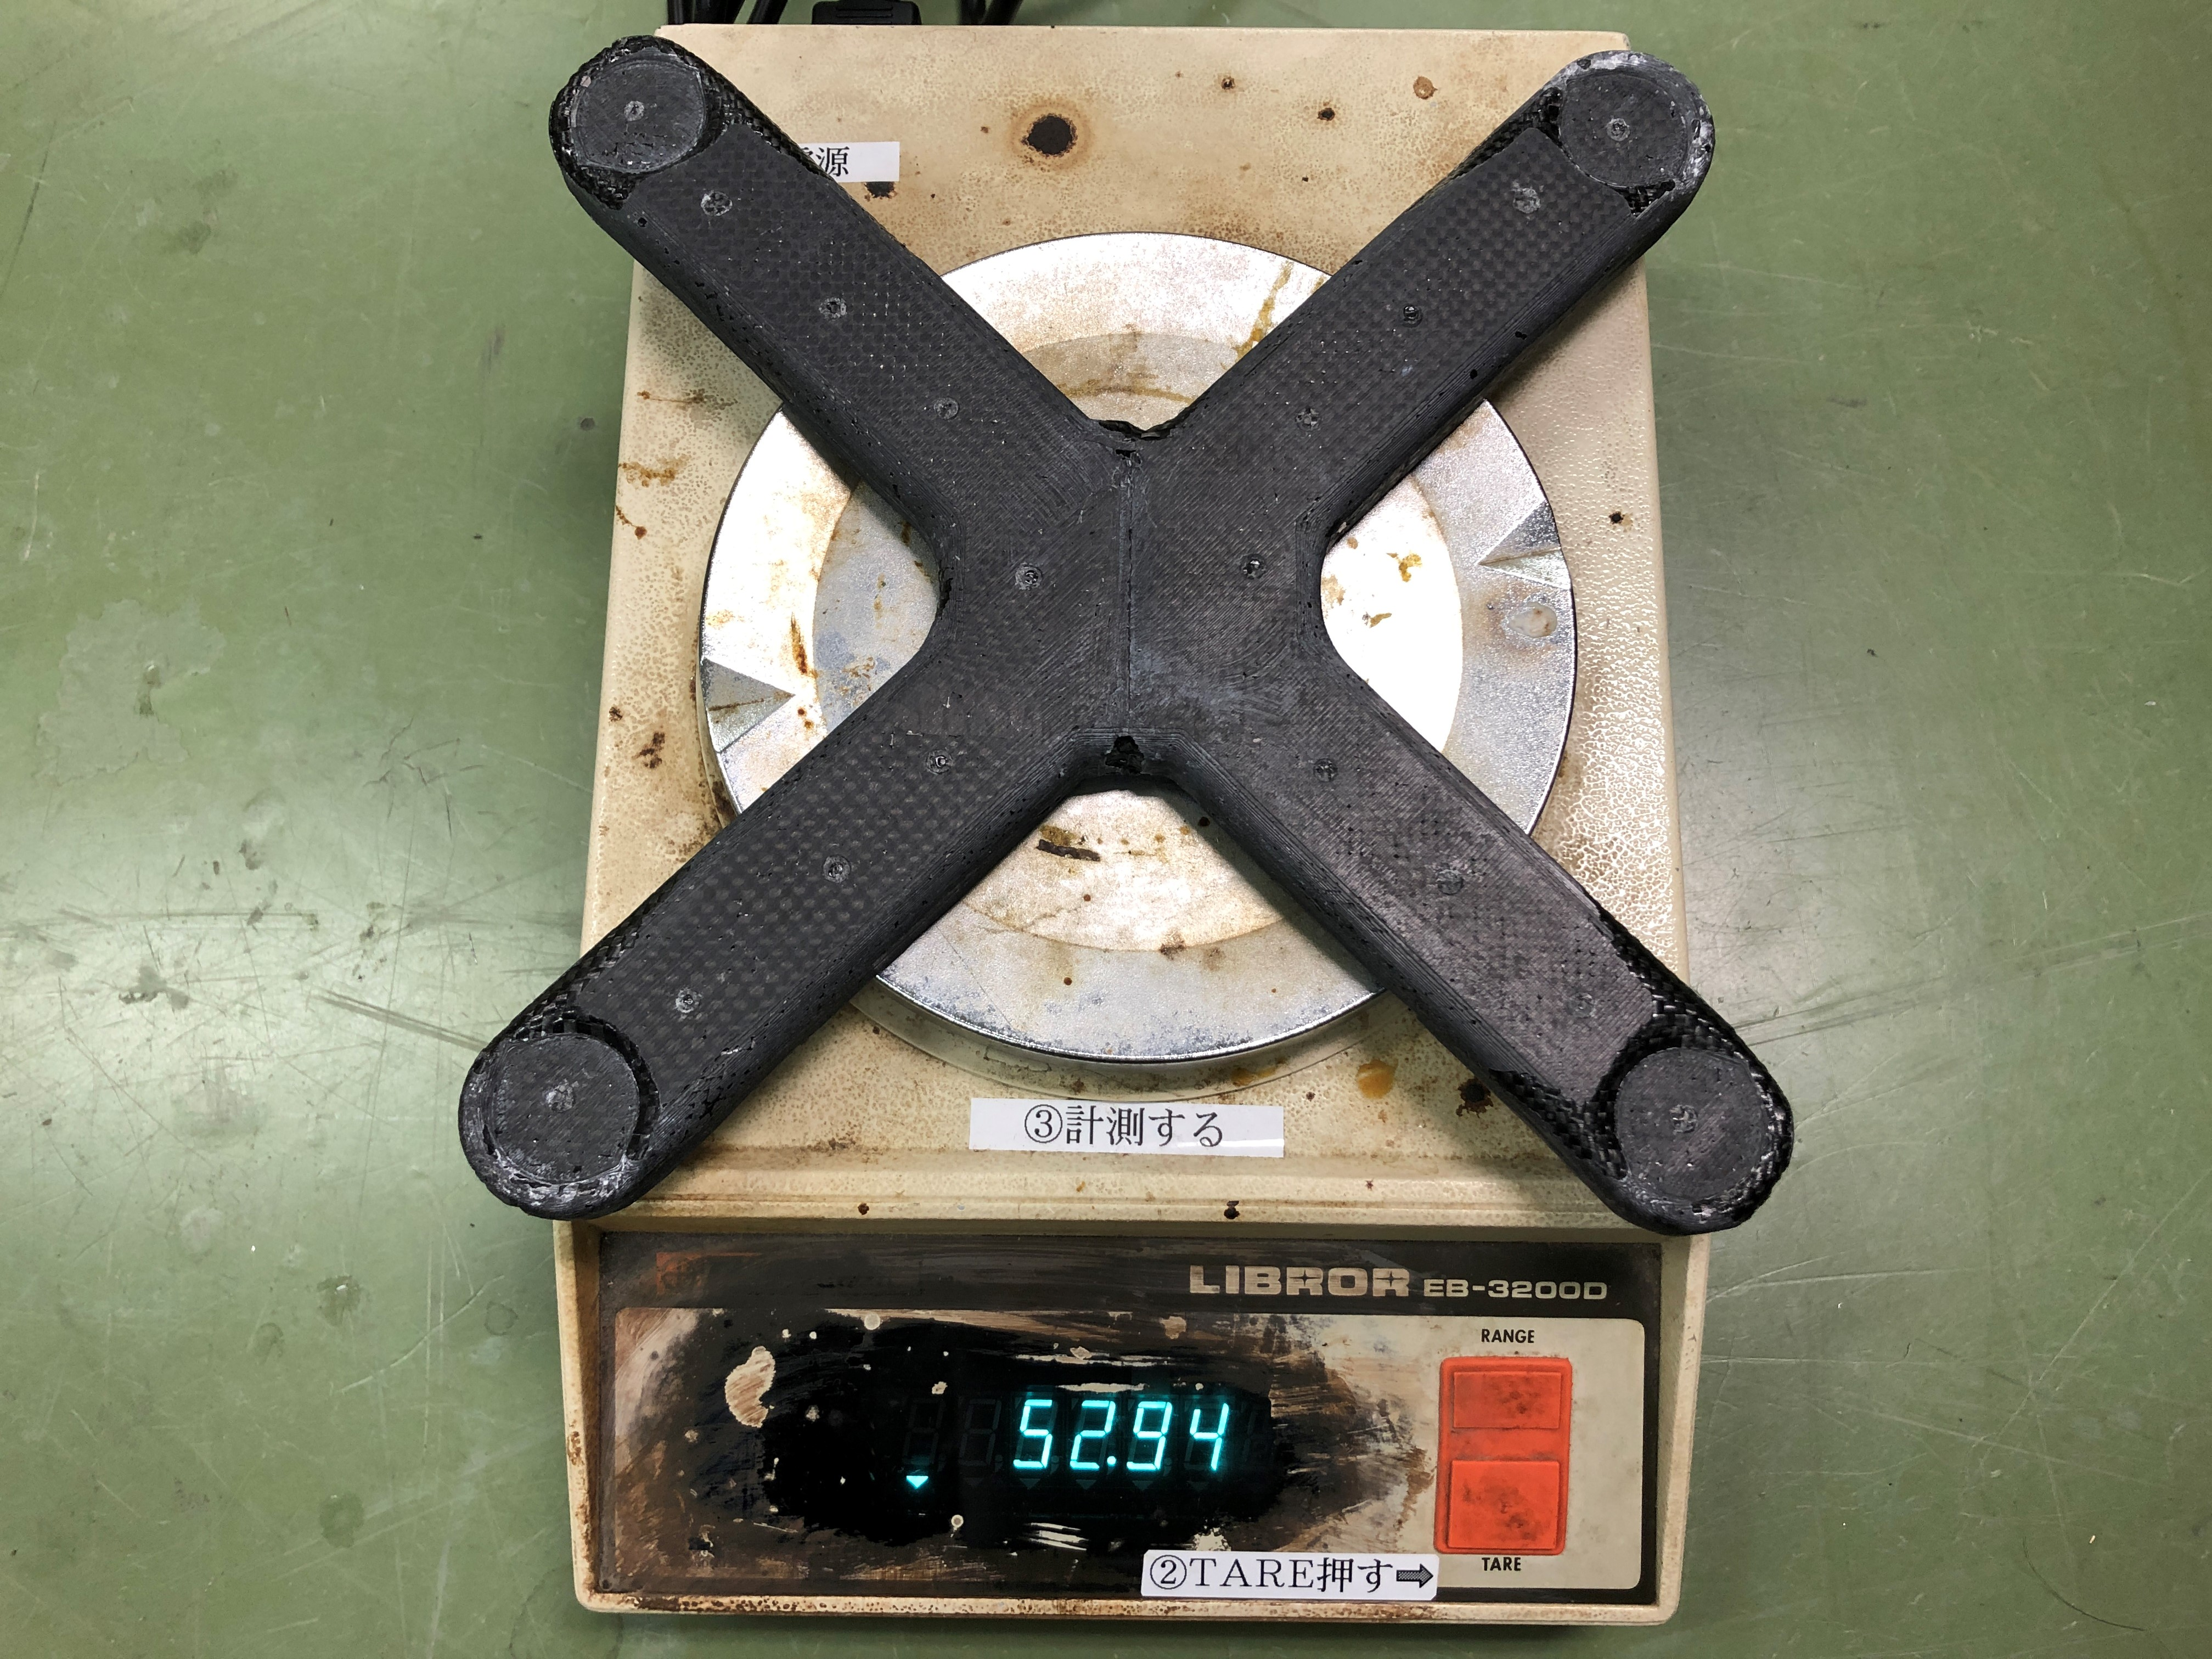
\includegraphics[width=50mm]{img/d.jpg}
    \end{center}
  \caption{完成した試作フレーム}
 \label{fig:a}
\end{figure}

\section{立体フレームの製作}
立体フレームを成型するための型は,3DCADにて設計を行い3Dプリンターを用いて製作を行った.

\subsection{プリンターでの立体型造形}
3Dプリンターでの造形には,各型につきそれぞれ6時間から7時間を要した.立体型は雄型,雌型をそれぞれの設計を行った.平面用の木枠は一体型に対し,立体フレーム用の型は大きさの関係上,造形時のプリンターのテーブルに収まらないため二つのパーツに分けて設計をした.積層時に連結するための突起部分も設計されている.また,造形時プリンターのノズルからの樹脂の射出温度と空冷時の室内温度の温度差が大きくなってしまう場合があった.その結果,反りが発生してしまい造形途中でクラックが入ったり,土台がテーブルから浮いてしまうなど,全体のゆがみの原因となってしまった.そのため造形時の土台の表面積を増加させ,テーブルにはのりを付着させそれらの防止をする工夫を施した.

\subsection{立体型への離型剤塗り付け作業}
立体フレーム用の型には離型剤として,車用のワックスを利用した.むらができてしまうと離型が困難になってしまうため,ワックスは厚めにぬりこんだ.また圧縮用のポリ袋にはくっつかず容易に離型することができる.

\subsection{積層作業}
離型剤を塗った型にカーボンシートをかぶせ,積層を行っていく.この際に一枚をフレームの形におおいかぶせるとしわができてしまったりと困難なため,四分割にして行った.型内部の縁に沿って折り目をつけていき,エポキシ樹脂を刷毛で塗っていく.二枚目以降も同様に積層作業を行い,隙間やエッジ部分のしわを極力少なくしてゆく.またカーボンシート枚数を重ねるごとにエポキシ樹脂の量を減少させていく.


\subsection{真空引き作業}
圧縮作業には,吸引機として掃除機とビニールポリ袋を用いて作業行った.積層作業を終えたものをビニールポリ袋に入れる.その後吸引のためのノズルを通す部分以外をアイロンで温め溶着させる.その後掃除機で圧縮作業を行っていく.圧縮の際に一気に空気を抜いていくのではなく,徐々に空気量を調整していきながらポリ袋を型の形に添わせながら空気を抜いてゆく.また型の角がポリ袋を傷つけないかを気を付けながら完全に空気を抜いていく.最終的にノズルを抜いていき,すべてを抜ききる手前でアイロンで溶着をさせ圧縮作業が完了する.

\subsection{バリ取り,ヤスリ掛け}
24時間以上が経過し完全移行化したフレームは,型から取り外しバリを糸ノコで切り落とし,やすり掛けを行い完成となる.


\section{平面フレームと立体フレーム強度比較}
平面フレームと立体フレームにおいてアームの強度試験を行った.試験方法としてアーム中央部の根元を固定し,モータ取り付け部の先端部分に,重さの違うおもりをつるしたわみ量を計測した.図3に示すグラフのように,平面フレームに比べ立体フレームの方が合成が高いことがわかる.平面体に比べ立体の方が,断面二次モーメントが大きいため合成が向上する.

\begin{figure}[htbp]
  \begin{center}
    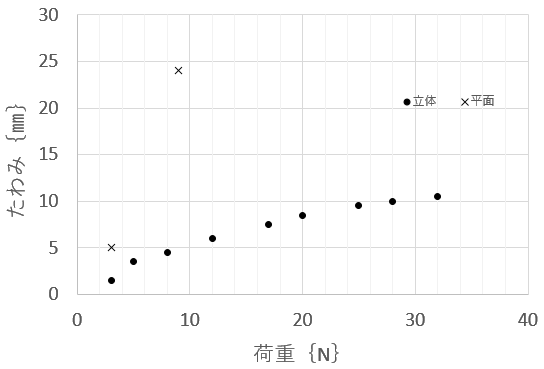
\includegraphics[width=55mm]{img/graph.png}
    \end{center}
  \caption{荷重・たわみ線図}
 \label{fig:a}
\end{figure}

\section{おわりに}
平面から立体フレームにすることで,積層枚数を減らすことができより軽量で剛性のあるフレームを製作する事ができる.またより厳密な質量管理を行うために,積層前に樹脂,カーボンクロスの質量を図っておくことでより完成後の質量を推測し,より厳密に制作が行えるだろう.

\section{参考文献}
①Fibreglass/FRP 2014/5/6
https://www.youtube.com/watch?v=keBwRhkfuOQ
②HowToMakeYourOwnCarbonFiberParts 2008/11/20
https://www.youtube.com/watch?v=IAdVO8Rkv6c



\end{document}